% このファイルの文字コードは UTF-8
% 環境はtexlive2018
%\documentclass[11pt, a4paper]{ujreport} %イキッてuplatexを使っているだけなので
\documentclass[11pt, a4paper]{jreport} %普通にplatexのこっちでいいと思われる(違いが知りたければggってください)
\usepackage[dvipdfmx]{graphicx} %画像読み込み用 texの壁なのでggって,どうぞ
\usepackage{thesis} % ここで表紙のテンプレ他を作ってる
\usepackage{here} %個人的に必須だと思っている.これがあると画像表示のとき[H]が使えるようになる.(その場所に画像を置く)
% 参考文献のとこで使う
\renewcommand{\bibname}{参考文献}


%タイトル
\title{タイトル}
\author{名前}
\date{平成〇年〇月〇日} 

\begin{document}
\maketitle

%概要
\begin{abstract}
概要
\end{abstract}

%目次
\tableofcontents
% 本文

%%%%%%%%%%%%%%%%%%%%%%%%%%%%%%%%%%%%%%%%%%%%%%%%%%%%%%%%%%%%%%%%%
% 1章 序論
%%%%%%%%%%%%%%%%%%%%%%%%%%%%%%%%%%%%%%%%%%%%%%%%%%%%%%%%%%%%%%%%%
\chapter{序論}
序論

%%%%%%%%%%%%%%%%%%%%%%%%%%%%%%%%%%%%%%%%%%%%%%%%%%%%%%%%%%
%2章
%%%%%%%%%%%%%%%%%%%%%%%%%%%%%%%%%%%%%%%%%%%%%%%%%%%%%%%%%%
\chapter{関連研究}

%%%%%%%%%%%%%%%%%%%%%%%%%%%%%%%%%%%%%%%%%%%%%%%%%%%%%%%%%%
% 2.1節
%%%%%%%%%%%%%%%%%%%%%%%%%%%%%%%%%%%%%%%%%%%%%%%%%%%%%%%%%%

\section{ご注文はうさぎですかという作品がもたらした幸福}

% 表のテスト
\begin{table}[H]
	\begin{center}
		\caption{表テスト}
		\begin{tabular}{|c||c|c|}
			\hline
			名前 & 誕生日 & 血液型\\
			\hline
			\hline
			ココア & 4月10日 & B型\\
			\hline
			チノ & 12月4日 & AB型\\ \hline
			リゼ & 2月14日 & A型\\ \hline
			千夜 & 9月19日 & O型\\ \hline
			シャロ & 7月15日 & A型\\ \hline
		\end{tabular}
	\end{center}
\end{table}


%%%%%%%%%%%%%%%%%%%%%%%%%%%%%%%%%%%%%%%%%%%%%%%%%%%%%%%%%%%%%%%%%
% 3章
%%%%%%%%%%%%%%%%%%%%%%%%%%%%%%%%%%%%%%%%%%%%%%%%%%%%%%%%%%%%%%%%%
\chapter{ごちうさキャラの実装}

%%%%%%%%%%%%%%%%%%%%%%%%%%%%%%%%%%%%%%%%%%%%%%%%%%%%%%%%%%%%%%%%%
% 3.1節
%%%%%%%%%%%%%%%%%%%%%%%%%%%%%%%%%%%%%%%%%%%%%%%%%%%%%%%%%%%%%%%%%
\section{ごちうさの概要}
概要
\subsection{テスト}
テスト\cite{gochiusa}
\begin{quote}
	引用例
\end{quote}

%%%%%%%%%%%%%%%%%%%%%%%%%%%%%%%%%%%%%%%%%%%%%%%%%%%%%%%%%%%%%%%%%
%4章 実験
%%%%%%%%%%%%%%%%%%%%%%%%%%%%%%%%%%%%%%%%%%%%%%%%%%%%%%%%%%%%%%%%%
\chapter{実験}
実験

% 画像の貼り方の1例.latexのエラーの原因は基本画像関連.
\begin{figure}[H]
	\centering
	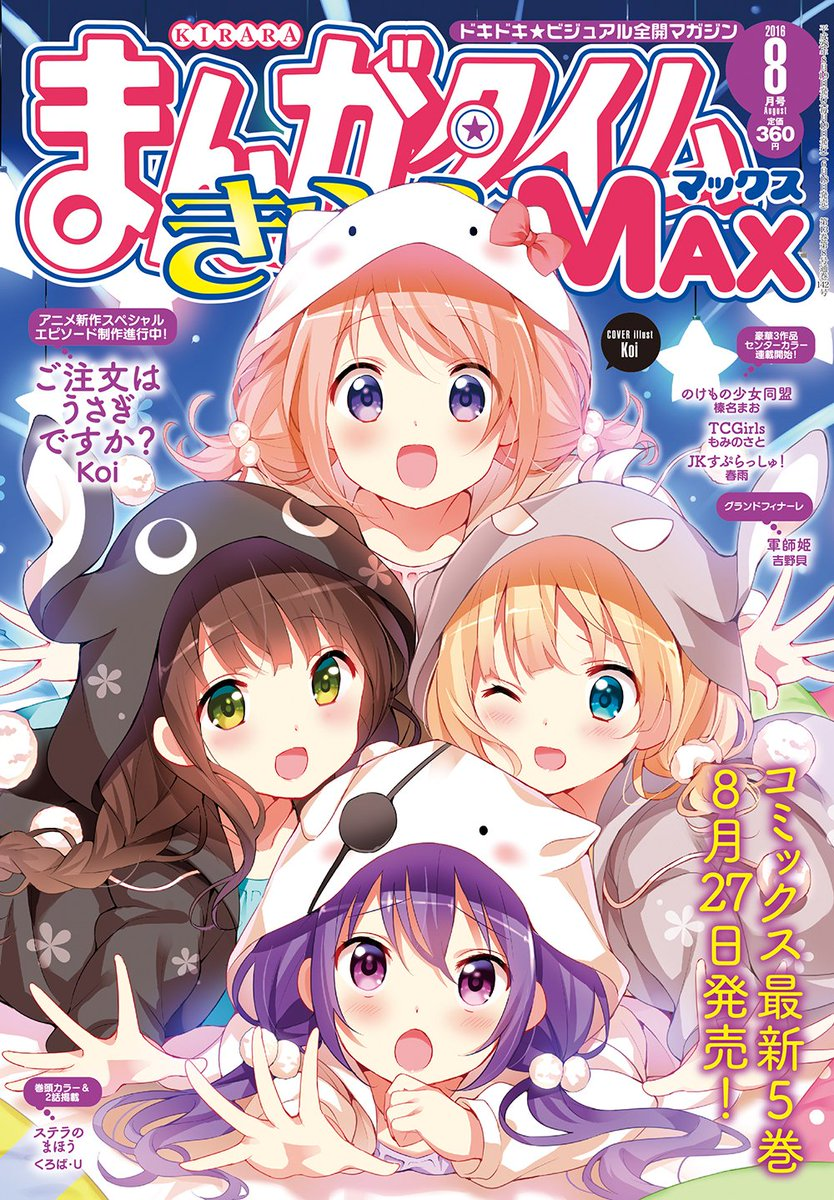
\includegraphics[width=0.7\linewidth]{example.jpg}
	\caption{画像のテスト}
	\label{fig:example}
\end{figure}

%%%%%%%%%%%%%%%%%%%%%%%%%%%
%結論
%%%%%%%%%%%%%%%%%%%%%%%%%%%
\chapter{結論}
結論

%%%%%%%%%%%%%%%%%%%%%%%%%%%
%謝辞
%%%%%%%%%%%%%%%%%%%%%%%%%%%
\chapter*{謝辞}
\addcontentsline{toc}{chapter}{謝辞}%目次に表示するためのやつ
謝辞

%%%%%%%%%%%%%%%%%%%%%%%%%%%
%参考文献
%%%%%%%%%%%%%%%%%%%%%%%%%%%
\bibliographystyle{junsrt}%参考文献を番号順に
\bibliography{bunken} %bunken.bibを参照している
\addcontentsline{toc}{chapter}{\bibname}%目次に表示するためのやつ

\end{document}